\documentclass{article}
\usepackage[margin=1in]{geometry}
\usepackage{amsmath}
\usepackage{amssymb}
\usepackage{graphicx}

\title{The Korteweg--de Vries equation: nonlinearity balances dispersion in shallow water}
\author{Holden Leslie-Bole}
\date{July 2023}

\begin{document}

\maketitle

\paragraph{How to read this note.} If you are seeing the KdV equation for the first time, one effective pass is: (i) read the boxed equations and the soliton plot in \S 6, (ii) track the two small parameters \(\epsilon\) (shallowness) and \(\delta\) (amplitude) as they propagate through the derivation, and then (iii) return for the algebraic details. The crux is the moment in \S 4 where the third-derivative term comes in.

\paragraph{The setting.} In August 1834, the Scottish engineer John Scott Russell was riding alongside the Union Canal near Edinburgh when a boat being towed by a pair of horses suddenly stopped. The displaced bow water did not break or disperse. As Russell later wrote, it
\begin{quote}
``rolled forward with great velocity, assuming the form of a large solitary elevation, a rounded, smooth, and well-defined heap of water, which continued its course along the channel apparently without change of form or diminution of speed.''
\end{quote}
He chased it on horseback at eight or nine miles an hour for a mile or two before he lost it in a bend of the canal. He called it the \emph{Wave of Translation}. The puzzle was sharp: water waves are supposed either to spread (because long components travel faster than short ones, so a localised pulse should disperse) or to steepen and break (because higher water travels faster than lower water, so a smooth profile should sharpen at the front). Russell's wave did neither.

\paragraph{The question.} Sixty years later, Diederik Korteweg and Gustav de Vries showed that for a shallow basin, the steepening and the spreading can be made to balance exactly. The resulting equation, in canonical non-dimensional form, is
\begin{equation}
\boxed{\;\eta_t + 6\, \eta\, \eta_x + \eta_{xxx} = 0.\;}
\label{eq:kdv-canonical}
\end{equation}
The first nonlinear term causes peaks to move faster than troughs (steepening); the third-derivative term causes long wavelengths to move faster than short ones (dispersion). Russell's solitary wave is the \(\mathrm{sech}^2\) profile that emerges as the exact equilibrium between the two, and we will derive it in \S 6.

This note traces the derivation of \eqref{eq:kdv-canonical} from the incompressible Euler equations on a flat-bottomed shallow basin. The chain is
\[
\text{Euler} \;\longrightarrow\; \text{linear shallow-water} \;\longrightarrow\; \text{KdV},
\]
with one perturbation expansion at each arrow.\footnote{The style of this note follows the conventions established in my earlier mean-field hydrodynamics note, which draws on W.R. Young's \emph{Mainly advection and diffusion} for the prose and F. Feddersen's \emph{Notes on Nearshore Physical Oceanography} for the structural scaffolding. I wrote the original handwritten version of this derivation in 2022; this is a clean re-write.}

\paragraph{Background assumed.} Multivariable calculus, ordinary and partial differential equations, and exposure to fluid mechanics at the level of the incompressible Euler equations. The two small parameters and the perturbation expansion are introduced as we go.

\paragraph{Notation.} \(x\) and \(z\) are horizontal and vertical Cartesian coordinates with \(z\) measured upward from the undisturbed water surface, and \(t\) is time. \(\eta(x,t)\) is the free-surface elevation. \(u(x,z,t)\) and \(w(x,z,t)\) are the horizontal and vertical components of the fluid velocity; \(p(x,z,t)\) is the pressure. \(h_0\) is the undisturbed water depth, \(a\) is a typical wave amplitude, and \(\lambda\) is a typical wavelength. \(g\) is gravitational acceleration, \(\rho\) is the (constant) fluid density, and \(c \equiv \sqrt{g h_0}\) is the linear long-wave speed. The two dimensionless small parameters are
\[
\epsilon \;\equiv\; \frac{h_0}{\lambda} \quad \text{(shallowness)}, \qquad
\delta \;\equiv\; \frac{a}{h_0} \quad \text{(amplitude)}.
\]

\paragraph{KdV scaling.} The two small parameters are independent in principle. The \emph{KdV regime} is the special case
\[
\delta \;=\; O(\epsilon^2),
\]
and we will see in \S 4 that this particular scaling is exactly what brings nonlinearity and dispersion to the same order.

\section*{1. Setup}

Consider an inviscid, incompressible fluid of constant density \(\rho\) in two dimensions \((x, z)\), with gravity acting in the \(-z\) direction. The fluid lies between a flat rigid bed at \(z = -h_0\) and a free surface at \(z = \eta(x,t)\), and is initially at rest. The governing equations are the incompressible Euler equations:
\begin{subequations}
\label{eq:euler}
\begin{align}
\partial_t u + u\, \partial_x u + w\, \partial_z u &= -\frac{1}{\rho}\, \partial_x p, \\
\partial_t w + u\, \partial_x w + w\, \partial_z w &= -\frac{1}{\rho}\, \partial_z p \;-\; g, \\
\partial_x u + \partial_z w &= 0.
\end{align}
\end{subequations}
Three boundary conditions complete the problem. At the rigid bed, no flow can pass through:
\begin{equation}
w = 0 \quad \text{at } z = -h_0.
\label{eq:bed}
\end{equation}
At the free surface \(z = \eta\), a fluid particle on the surface must remain on the surface (kinematic condition):
\begin{equation}
\partial_t \eta + u\, \partial_x \eta = w \quad \text{at } z = \eta.
\label{eq:kinematic}
\end{equation}
And the pressure on the free surface equals atmospheric pressure, which we absorb into \(p\) and set to zero (dynamic condition):
\begin{equation}
p = 0 \quad \text{at } z = \eta.
\label{eq:dynamic}
\end{equation}
We have dropped viscosity from the start. For the long-wavelength small-amplitude regime that produces KdV, the viscous terms are smaller than the dispersive correction by a factor of \(O(\epsilon^2/\mathrm{Re})\) and play no leading role.

\noindent\emph{Intuition.} A wave passes by; what's the typical horizontal scale of the disturbance? \(\lambda\). What's the typical vertical scale? \(h_0\). What's the typical surface displacement? \(a\). The KdV regime is the case where \(a \ll h_0 \ll \lambda\) with the specific relationship \(a/h_0 \sim (h_0/\lambda)^2\).

\section*{2. Non-dimensionalization}

Rescale the variables using the natural scales \(\lambda\), \(h_0\), \(\lambda/c\), \(a\), and the leading-order linear-wave estimates for velocity and pressure. Specifically, let
\begin{equation}
x = \lambda x', \quad z = h_0 z', \quad t = \frac{\lambda}{c} t', \quad
\eta = a \eta', \quad
u = \delta c\, u', \quad
w = \delta \epsilon c\, w',
\label{eq:scales}
\end{equation}
and split the pressure into a hydrostatic background plus a dynamic correction:
\begin{equation}
p = -\rho g z + \rho g a\, \tilde p,
\label{eq:psplit}
\end{equation}
so that \(\tilde p\) is dimensionless and \(O(1)\). The horizontal velocity scale \(\delta c\) is what the linear shallow-water solution gives (\S 3); the vertical velocity scale \(\delta \epsilon c\) is the value forced by continuity.

Substituting \eqref{eq:scales}--\eqref{eq:psplit} into the Euler equations \eqref{eq:euler} and dropping the primes, the non-dimensional system is:
\begin{subequations}
\label{eq:nondim}
\begin{align}
\partial_t u + \delta\, (u\, \partial_x u + w\, \partial_z u) &= -\partial_x \tilde p, \label{eq:nondim-x} \\
\epsilon^2\!\left[\partial_t w + \delta\, (u\, \partial_x w + w\, \partial_z w)\right] &= -\partial_z \tilde p, \label{eq:nondim-z} \\
\partial_x u + \partial_z w &= 0. \label{eq:nondim-cont}
\end{align}
\end{subequations}
The boundary conditions become:
\begin{align}
w &= 0 \quad \text{at } z = -1, \label{eq:nd-bed} \\
\partial_t \eta + \delta\, u\, \partial_x \eta &= w \quad \text{at } z = \delta \eta, \label{eq:nd-kin} \\
\tilde p &= \eta \quad \text{at } z = \delta \eta. \label{eq:nd-dyn}
\end{align}

\noindent\emph{Intuition.} The two small parameters appear in distinct places: \(\delta\) tags every nonlinear (advective) term, and \(\epsilon^2\) tags only the vertical-acceleration term in z-momentum. In the \(\epsilon, \delta \to 0\) limit we get a linear equation; the \(\delta\) and \(\epsilon^2\) corrections will respectively introduce nonlinearity and dispersion.

\section*{3. Leading order: linear shallow water}

Set \(\delta = 0\) and \(\epsilon = 0\) in \eqref{eq:nondim}--\eqref{eq:nd-dyn}.

The z-momentum equation becomes \(\partial_z \tilde p = 0\), so \(\tilde p\) is independent of \(z\). The dynamic surface condition \eqref{eq:nd-dyn} gives \(\tilde p = \eta\) at \(z = 0\), and so
\begin{equation}
\tilde p(x, z, t) = \eta(x, t) \quad \text{at leading order}
\label{eq:LO-p}
\end{equation}
throughout the depth. This is the hydrostatic statement: the dynamic pressure at any depth equals the surface elevation above it.

The x-momentum equation \eqref{eq:nondim-x} reduces to \(\partial_t u = -\partial_x \tilde p = -\partial_x \eta\). Since the right-hand side is independent of \(z\), the velocity \(u\) remains \(z\)-independent if it starts that way: \(u = U(x, t)\). Then
\begin{equation}
\partial_t U = -\partial_x \eta.
\label{eq:LO-mom}
\end{equation}

Continuity \eqref{eq:nondim-cont} gives \(\partial_z w = -\partial_x U\), and integrating from the bed (where \(w=0\)) yields
\begin{equation}
w(x, z, t) = -(z + 1)\, \partial_x U.
\label{eq:LO-w}
\end{equation}
At the surface, \(w(x, 0, t) = -\partial_x U\). The kinematic condition \eqref{eq:nd-kin} at leading order is \(\partial_t \eta = w(x, 0, t)\), giving
\begin{equation}
\partial_t \eta = -\partial_x U.
\label{eq:LO-cont}
\end{equation}

Equations \eqref{eq:LO-mom} and \eqref{eq:LO-cont} are the \emph{linear shallow-water} equations. Combining them gives the classical wave equation \(\partial_t^2 \eta = \partial_x^2 \eta\). The general solution is a sum of right-going and left-going waves; for a right-going wave,
\begin{equation}
\eta = U = f(x - t)
\label{eq:right-going}
\end{equation}
for any localised initial profile \(f\), with non-dimensional speed \(c = 1\) (dimensional \(\sqrt{g h_0}\)).

\noindent\emph{Intuition.} At leading order the surface and the depth-uniform horizontal velocity propagate together as non-dispersive linear waves. There is no steepening (no nonlinearity yet), and there is no dispersion (no third-derivative term yet). To capture Russell's solitary wave, we have to go to the next order.

\section*{4. Next order: where nonlinearity and dispersion come in}

Now retain both \(\delta\) (nonlinearity) and \(\epsilon^2\) (dispersion). Under the KdV scaling \(\delta = O(\epsilon^2)\), they enter the same equation at the same order.

\subsection*{4.1 The non-hydrostatic pressure correction}

The leading-order pressure was hydrostatic because we set \(\epsilon^2 = 0\) in z-momentum. Restoring it, \eqref{eq:nondim-z} gives at next order
\begin{equation}
\partial_z \tilde p = -\epsilon^2\, \partial_t w + O(\delta \epsilon^2, \epsilon^4).
\label{eq:NLO-pz}
\end{equation}
Use the leading-order \(w\) from \eqref{eq:LO-w}. Then \(\partial_t w = -(z+1)\partial_x \partial_t U = (z+1)\, \partial_x^2 \eta\), where the second equality uses \eqref{eq:LO-mom}. Substituting,
\[
\partial_z \tilde p = -\epsilon^2\, (z+1)\, \partial_x^2 \eta.
\]
Integrate from \(z\) up to the surface (\(z = 0\) at this order), using \(\tilde p(x, 0, t) = \eta\):
\begin{equation}
\tilde p(x, z, t) = \eta(x, t) - \frac{\epsilon^2}{2}\,\bigl[1 - (z+1)^2\bigr]\, \partial_x^2 \eta(x, t) + O(\delta).
\label{eq:p-correction}
\end{equation}
The pressure is no longer purely hydrostatic: a parcel of fluid undergoing vertical acceleration pushes against the surrounding pressure field, and the second-derivative term \(\partial_x^2 \eta\) is the resulting depth-dependent correction.

\subsection*{4.2 Depth-averaged equations}

Average each equation in \eqref{eq:nondim} over the fluid column, \(\langle \phi \rangle \equiv \int_{-1}^{0} \phi\, dz\) (with the surface at \(z = \delta \eta \approx 0\) at this order). Using \(u = U(x,t)\) at leading order and the pressure profile \eqref{eq:p-correction}, one finds
\[
\langle \tilde p \rangle = \eta - \frac{\epsilon^2}{2} \langle 1 - (z+1)^2 \rangle\, \partial_x^2 \eta = \eta - \frac{\epsilon^2}{3}\, \partial_x^2 \eta,
\]
where \(\langle 1 - (z+1)^2 \rangle = 2/3\). The depth-averaged x-momentum equation is then
\begin{equation}
\partial_t U + \delta\, U\, \partial_x U + \partial_x \eta = \frac{\epsilon^2}{3}\, \partial_x^3 \eta + O(\delta^2, \epsilon^4).
\label{eq:boussinesq-mom}
\end{equation}
The depth-integrated continuity equation, using the kinematic surface condition \eqref{eq:nd-kin} to eliminate \(w\) at \(z = \delta \eta\), is
\begin{equation}
\partial_t \eta + \partial_x\!\left[(1 + \delta \eta)\, U\right] = 0.
\label{eq:boussinesq-cont}
\end{equation}

Equations \eqref{eq:boussinesq-mom} and \eqref{eq:boussinesq-cont} are a pair of \emph{Boussinesq-type} equations: they retain the leading nonlinearity (\(U\,\partial_x U\) and \((\eta U)_x\)) and the leading dispersion (\((\epsilon^2/3)\, \partial_x^3 \eta\)). They are valid to first order in both small parameters.

\noindent\emph{Intuition.} Notice the asymmetry. Nonlinearity appears in both equations: the advection of momentum in \eqref{eq:boussinesq-mom}, and the finite-amplitude factor \((1 + \delta \eta)\) in continuity \eqref{eq:boussinesq-cont}. Dispersion appears only in the momentum equation, and only in the form of the depth-integrated non-hydrostatic pressure correction. KdV is what these equations reduce to once a unidirectional wave is selected.

\subsection*{4.3 Reduction to KdV by selecting a right-going wave}

At leading order, \(U = \eta\) for a right-going wave \eqref{eq:right-going}. Allow corrections of order \(\delta\) and \(\epsilon^2\),
\[
U = \eta + \delta\, U_a(x, t) + \epsilon^2\, U_b(x, t) + \cdots,
\]
and substitute into \eqref{eq:boussinesq-mom}--\eqref{eq:boussinesq-cont}. Adding the two equations cancels the leading-order \((\partial_t \eta + \partial_x \eta)\) and isolates the \(O(\delta, \epsilon^2)\) corrections. Subtracting them, and using the leading-order relation \(\partial_t \approx -\partial_x\) for right-going components, fixes \(U_a\) and \(U_b\) up to the slow evolution. The result, in the original variables and restoring the dimensional constants, is the dimensional KdV equation
\begin{equation}
\boxed{\;
\partial_t \eta + c\, \partial_x \eta + \frac{3 c}{2 h_0}\, \eta\, \partial_x \eta + \frac{c\, h_0^2}{6}\, \partial_x^3 \eta = 0.
\;}
\label{eq:kdv-dimensional}
\end{equation}
The four terms are: time evolution, linear advection at the long-wave speed \(c\), nonlinear self-steepening with coefficient \(3c/(2h_0)\), and dispersion with coefficient \(c h_0^2/6\). Going into a frame moving at the leading-order wave speed (\(X = x - c t\)), the linear advection term vanishes; rescaling \(\eta\), \(X\), and \(t\) appropriately then collapses the two remaining coefficients into the canonical form \eqref{eq:kdv-canonical}.

\section*{5. The KdV equation}

The dimensional equation \eqref{eq:kdv-dimensional} and its canonical reduction \eqref{eq:kdv-canonical} are the main result of the derivation. Two structural points are worth noting.

\paragraph{The balance.} Each of the three nonlinear/dispersive corrections in \eqref{eq:kdv-dimensional} is small (the wave amplitude is small compared to the depth, and the depth is small compared to the wavelength). The \emph{KdV regime} is exactly the special case where the nonlinear and dispersive corrections have comparable magnitudes. If \(a/h_0 \gg (h_0/\lambda)^2\), nonlinearity wins: the wave steepens and breaks (the equation reduces to inviscid Burgers). If \(a/h_0 \ll (h_0/\lambda)^2\), dispersion wins: the wave spreads (the equation reduces to a linear dispersive PDE). KdV lives on the curve where the two effects are equal.

\paragraph{Why ``canonical''.} The equation \eqref{eq:kdv-canonical} has the same shape as \eqref{eq:kdv-dimensional} once the dimensional coefficients have been absorbed into a redefinition of the variables. This is the form of the equation usually quoted in textbooks, and it is the form whose solutions we discuss next.

\section*{6. The soliton solution}

Look for a traveling-wave solution of the canonical KdV equation \eqref{eq:kdv-canonical}, i.e.\ a solution of the form \(\eta(x, t) = f(\xi)\) with \(\xi \equiv x - c t\). Substituting,
\[
- c\, f' + 6\, f f' + f''' = 0.
\]
Integrate once with respect to \(\xi\). Using the boundary conditions \(f, f' \to 0\) as \(|\xi| \to \infty\), the constant of integration vanishes:
\begin{equation}
- c\, f + 3\, f^2 + f'' = 0.
\label{eq:soliton-1}
\end{equation}
Multiply \eqref{eq:soliton-1} by \(f'\) and integrate again. The constant again vanishes, leaving
\begin{equation}
(f')^2 = c\, f^2 - 2\, f^3 = f^2\, (c - 2 f).
\label{eq:soliton-2}
\end{equation}
The right-hand side is non-negative only when \(0 \leq f \leq c/2\), so the wave is non-negative and reaches a maximum amplitude \(f_{\max} = c/2\) where \(f' = 0\).

Try the ansatz \(f(\xi) = (c/2)\, \mathrm{sech}^2(k \xi)\). Then
\[
f' = -c\, k\, \mathrm{sech}^2(k\xi)\, \tanh(k\xi), \qquad
(f')^2 = c^2\, k^2\, \mathrm{sech}^4(k\xi)\, \tanh^2(k\xi).
\]
Computing the right-hand side of \eqref{eq:soliton-2} for the same ansatz gives \(f^2(c - 2f) = (c^3/4)\, \mathrm{sech}^4(k\xi)\, \tanh^2(k\xi)\). Matching the two expressions fixes \(k^2 = c/4\), so \(k = \sqrt{c}/2\). The soliton solution is therefore
\begin{equation}
\boxed{\;
\eta(x, t) = \frac{c}{2}\, \mathrm{sech}^2\!\left(\frac{\sqrt{c}}{2}\,(x - c t)\right).
\;}
\label{eq:soliton}
\end{equation}

Equivalently, in terms of the amplitude \(A \equiv c/2\),
\[
\eta(x, t) = A\, \mathrm{sech}^2\!\left(\sqrt{\tfrac{A}{2}}\,(x - 2 A\, t)\right).
\]

\paragraph{The amplitude--speed relation.} The soliton speed is \(c = 2A\): \emph{taller solitons travel faster}. The soliton width is \(1/\sqrt{A/2} = \sqrt{2/A}\): \emph{taller solitons are also narrower}. A small soliton is a long, slow bump; a large soliton is a tall, narrow, fast pulse. Both translate without changing shape, because nonlinear self-steepening and linear dispersion exactly cancel.

\begin{figure}[h!]
\centering
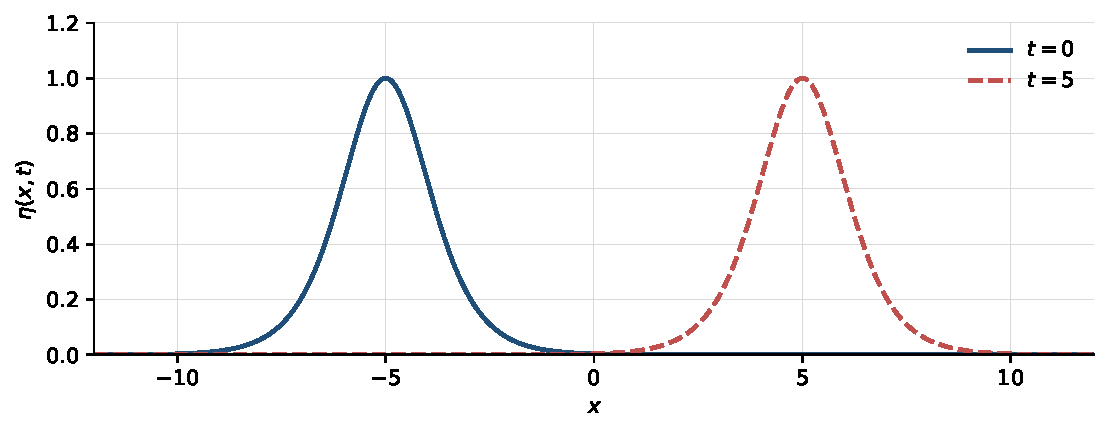
\includegraphics[width=0.85\textwidth]{soliton.pdf}
\caption{The single-soliton solution \eqref{eq:soliton} for amplitude \(A = 1\) and speed \(c = 2 A = 2\), shown at \(t = 0\) (solid blue) and \(t = 5\) (dashed red). The peak has translated by \(c\, \Delta t = 10\) units to the right, with the profile exactly preserved.}
\label{fig:soliton}
\end{figure}

\section*{7. What this explains}

\paragraph{Russell's wave.} The amplitude--speed relation \(c = 2A\) (in canonical units) makes Russell's observation a consistency statement. The wave he chased on horseback was a single soliton: an exact equilibrium between the steepening and spreading tendencies of small-amplitude long water waves, propagating at a speed set by its amplitude. Russell's wave could not have dispersed without being something other than a soliton.

\paragraph{Integrability.} The KdV equation is integrable. Any reasonable localised initial condition decomposes, as \(t \to \infty\), into a finite collection of solitons (sorted by speed, with the tallest at the front) plus a small dispersive tail. This was discovered by Gardner, Greene, Kruskal, and Miura in 1967, and the inverse-scattering method they introduced launched a whole field of integrable PDE theory. The note here only shows that the soliton exists; the deeper statement that \emph{everything} reduces to solitons is a separate result.

\paragraph{Where this leads.} The derivation given here is for surface waves on a single homogeneous fluid layer. The same machinery (small-amplitude, long-wavelength, balance of nonlinearity and dispersion) applies to internal waves in a stratified ocean, to interfacial waves between layers of different density, and to long waves on a sheared mean flow. The resulting evolution equations are KdV, the Gardner equation (when the quadratic nonlinear coefficient vanishes), the Benjamin--Ono equation (when the wave sits on a deep stratified layer), or the intermediate long-wave equation (for finite stratified depth). A separate note on those extensions, drawn from material in Falk Feddersen's advanced nonlinear-waves class, will follow.

\end{document}
